\section{Benchmark calculations}

\subsection{Independent Bernoulli thinning}

As an auxiliary normalization benchmark, enlarge the mark space by an
independent Bernoulli variable and take
$h\sim\operatorname{Bernoulli}(\pi)$ independently of the columns.  This is
not literally a deterministic function of the original $g$ unless that
independent coordinate is added; it is used only to check the factors of
$\pi$, $\phi$, and $\lambda$.  Then
\begin{equation}
M_d=\frac{N_d}{n}
\left(\frac1{N_d}A_+A_+^{\mathsf T}\right),
\qquad
\frac{N_d}{d}\to c=\phi\pi.
\end{equation}
The continuous bulk edges are
\begin{equation}
\lambda_\pm=
\frac{(1\pm\sqrt c)^2}{\lambda\phi}
=
\frac{\pi}{\lambda}
\left(1\pm\frac1{\sqrt c}\right)^2,
\end{equation}
and the zero mass is $(1-c)_+$. Equation \eqref{S:fixedpoint} becomes
\begin{equation}
zS(z)^2+
(1+\lambda\phi z-\phi\pi)S(z)+\lambda\phi=0.
\end{equation}

\subsection{Centered pure gate}

Let $Y=\lambda^{-1/2}Z$ with $Z\sim N(0,I_d)$ and
$h=\1_{\{\langle\ell,Z\rangle>0\}}$. Conditional on $ZZ^{\mathsf T}$, the only Gaussian preimages are $Z$ and $-Z$, with equal probability, and the gate takes complementary values. Therefore
\begin{equation}
\Pp\{h=1\mid YY^{\mathsf T}\}=\frac12,
\end{equation}
so $h$ is independent of $YY^{\mathsf T}$. The model is exactly independent Bernoulli thinning with $\pi=1/2$.

\subsection{Noncentered scalar gate}

Let $g\sim N(0,1)$,
\begin{equation}
h(g)=\1_{\{a+bg>0\}},\qquad b\ne0,
\end{equation}
and define
\begin{equation}
\delta=\frac a{|b|},\quad s_b=\operatorname{sign}(b),\quad
\pi=\Phi(\delta),\quad
\kappa=\frac{\varphi(\delta)}{\Phi(\delta)}.
\end{equation}
Then
\begin{equation}
\E[g\mid h=1]=s_b\kappa,\qquad
\E[g^2\mid h=1]=1-\delta\kappa.
\end{equation}
For $v=m+\lambda^{-1/2}g$, set
\begin{equation}
c=\phi\pi,\qquad
\beta=\lambda\E[v^2\mid h=1]
=\lambda m^2+2\sqrt\lambda\,m s_b\kappa+1-\delta\kappa.
\end{equation}
For the active $1/N_{\rm active}$ normalization, the effective scalar
matrix is
\begin{equation}
F_+(x)=\frac{c\beta}{\lambda c+s_+(x)},
\end{equation}
where $s_+$ solves
\begin{equation}
1+xs_+(x)=\frac{c\,s_+(x)}{\lambda c+s_+(x)}.
\end{equation}
At an effective root $x=F_+(x)$ these two equations imply
\begin{equation}
xs_+(x)=-\frac{\beta}{\beta-1},
\qquad
x=\frac{\beta}{\lambda}
\left(1+\frac1{c(\beta-1)}\right).
\end{equation}
This point lies strictly above the active Marchenko--Pastur edge
$\lambda^{-1}(1+c^{-1/2})^2$ exactly when
\begin{equation}
\beta>1+\frac1{\sqrt c}.
\end{equation}
Multiplication by the active fraction $\pi$ therefore gives
\begin{equation}
z_{\mathrm{out}}
=
\frac{\pi}{\lambda}\,
\beta\left(1+\frac1{c(\beta-1)}\right).
\end{equation}

\subsection{Fixed-\texorpdfstring{$\epsilon$}{epsilon} comparison}

For comparison only, define
\begin{equation}
D_\epsilon=D+\epsilon P_0,\qquad
P_0=\diag(\1_{\{D_{\ell\ell}=0\}}).
\end{equation}
Then
\begin{equation}
M_{d,\epsilon}-M_d
=\frac{\epsilon}{n}A_dP_0A_d^{\mathsf T}
\end{equation}
and
\begin{equation}
\|M_{d,\epsilon}-M_d\|
\le\epsilon\frac{\|A_d\|^2}{n}
=O_{\Pp}(\epsilon).
\end{equation}
This perturbation estimate does not, by itself, prove support-edge or root-multiplicity stability. The exact active reduction avoids that missing limit interchange.

\section{Reproducible numerical checks}
\label{S:numerical-section}

Figure~\ref{S:fig-noncentered} illustrates the scalar noncentered gate from the preceding subsection. It is a diagnostic rather than part of the proof.
\begin{figure}[t]
\centering
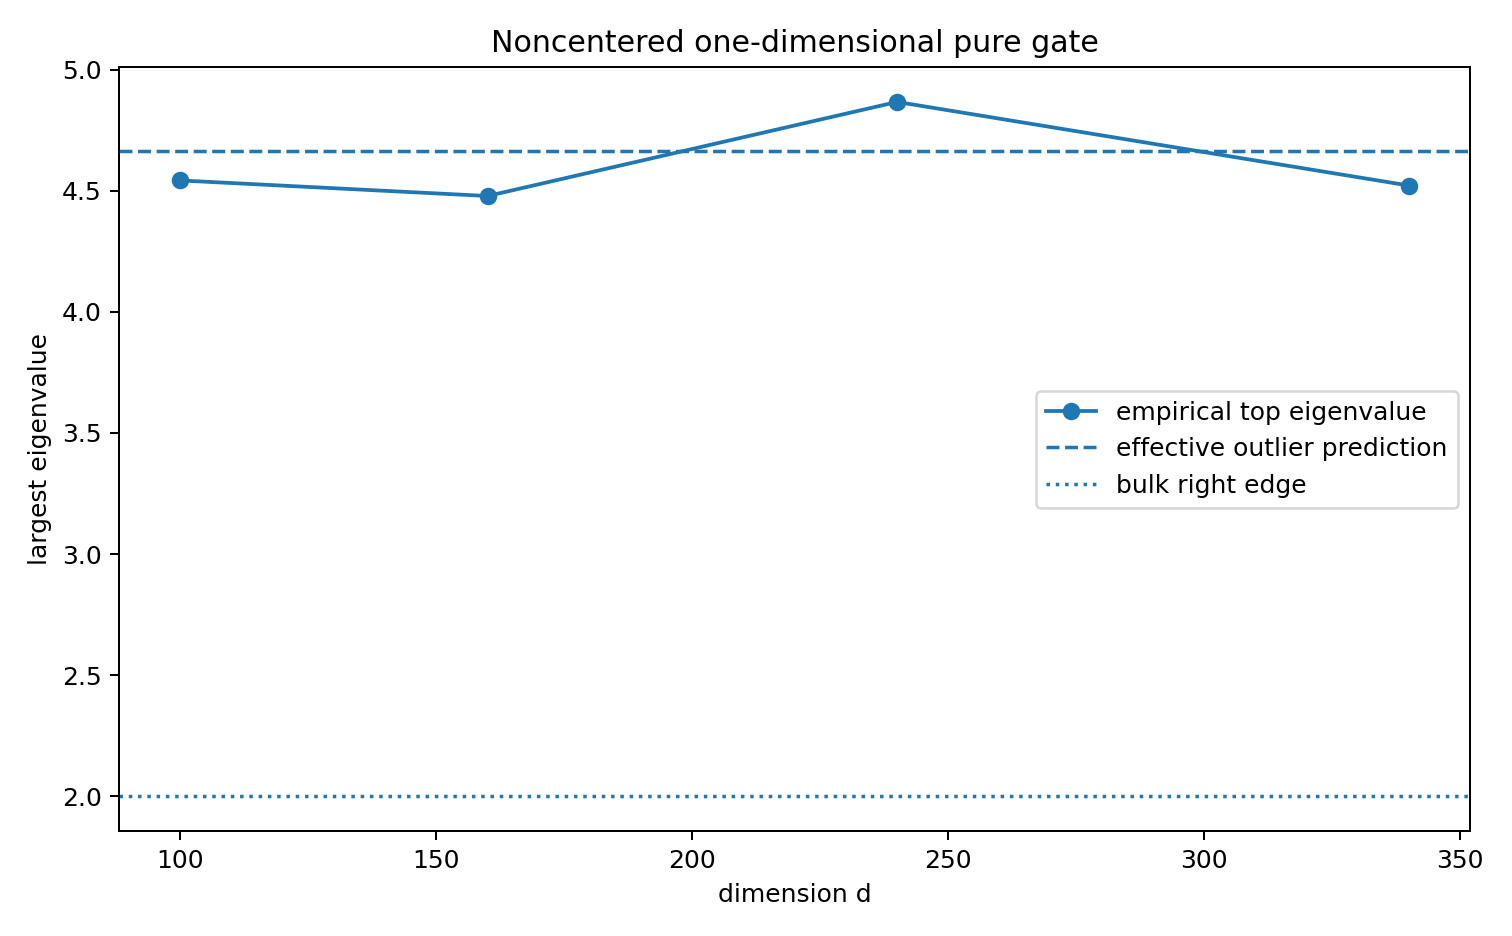
\includegraphics[width=0.86\linewidth]{figures/noncentered_outlier_check.png}
\caption{Largest empirical eigenvalue for $h(g)=\1_{\{g>0\}}$, $\phi=2$, $\lambda=1$, and summary mean $m=2$. The effective equation predicts $z_{\rm out}=4.6653$ and the bulk edge is $2$. Master seed: \texttt{20260720}.}
\label{S:fig-noncentered}
\end{figure}

The repository contains two executable Python scripts, fixed master seed
\texttt{20260720}, package versions, JSON output, and four plots. Representative checks are:
\begin{center}
\begin{tabular}{@{}ll@{}}
\toprule
Diagnostic & Recorded value\\
\midrule
Bernoulli model rank & $254$ observed, $254$ predicted\\
Bernoulli zero mass & $0.20625$ observed, $0.2$ limiting\\
Bernoulli top eigenvalue & $1.1641$ observed, $1.1963$ edge\\
Stieltjes residual & $2.39\times10^{-16}$\\
Centered gate top eigenvalue & $1.9728$, edge $2$\\
Noncentered predicted outlier & $4.6653$\\
Noncentered simulations & $4.48$--$4.87$\\
Determinant residual & $1.62\times10^{-10}$\\
Regularization identity error & $<1.1\times10^{-17}$\\
Two-construction operator difference & $1.93\times10^{-15}$\\
\bottomrule
\end{tabular}
\end{center}
These computations are diagnostic and do not replace the analytic proof.

\section{Proof dependency and failure-mode audit}

The logical dependency of the theorem is now explicit. The non-elementary
external inputs are the four source weighted-Wishart statements isolated in
Proposition~\ref{S:source-input}: bulk convergence, absence of outliers,
anisotropic resolvent control, and transform convergence. Every use of those
results occurs
after conditioning on the active marks and after checking independence,
strong empirical convergence of the weights, the positive gap $T\ge\tau$,
and fixed-dimensionality of the test vectors. The remaining dependencies are
proved in this manuscript: the conditional active law, exact Schur identities,
marked uniform law of large numbers, deterministic dilation, exact rank,
root multiplicity, random-size transfer, contour count, and spectral projection.

The proof dependency status is therefore:
\begin{description}
\item[Known external input.] The source bulk theorem and its
weighted-Wishart estimates: Propositions~2.7--2.8, Theorem~2.12, and
Lemma~2.13 of Ref.~\cite{BenArousEtAl2025}.
\item[Proved here.] The active conditional law and exact reduction
(Lemma~\ref{S:active-law-lemma} and \eqref{S:activeidentity}); the exact
Schur identities (Lemma~\ref{S:exact-schur-lemma}); the marked theorem
(Proposition~\ref{S:marked-theorem}); the dilation and zero atom
(\eqref{S:bulk-BL-transfer}--\eqref{S:pushforward} and
Lemma~\ref{S:zero-mass-lemma}); exact rank, root multiplicity, count
transfer, simple-root eigenvectors, and repeated-root projections.
\item[Computational diagnostic.] The deterministic numerical and
finite-dimensional identity checks in Section~\ref*{S:numerical-section}.  They are not used in
the proof.
\end{description}

For clarity, the principal failure modes are resolved as follows.
\begin{center}
\begin{tabular}{@{}p{0.30\linewidth}p{0.62\linewidth}@{}}
\toprule
Potential failure & Resolution \\
\midrule
Singular inverse & The inactive block is deleted before linearization; only $D_+^{-1}$ is used and $\|D_+^{-1}\|\le\tau^{-1}$. \\
Incorrect conditioning & The active law is the truncated/reweighted law \eqref{S:active-law}; it is never replaced by the original Gaussian mixture. \\
Lost normalization & $N_d/n$, $N_d/d$, and $N_d/(d-q)$ are kept distinct until their final limits. \\
Imported local law & Proposition~\ref{S:source-input} states the exact row-normalized equation; random test vectors may depend on $D$ but must be independent of the Gaussian block, exactly as in the source theorem. \\
Random-size bulk transfer & Weak convergence is metrized by $d_{\mathrm{BL}}$ before applying the random-index lemma; the later scaling uses the deterministic test $f(\pi x)$ and the trace bound \eqref{S:active-trace-bound}. \\
Weak support argument & The target bulk is the exact dilation \eqref{S:pushforward} of the active bulk. \\
Multiplicity loss & $B_G'(z)\succeq I$ and the kernel/complement expansion prove \eqref{S:multiplicity}; the argument principle then preserves analytic multiplicity. \\
Repeated eigenvalues & Only the full spectral projection \eqref{S:projection} is asserted; individual eigenvectors may rotate. \\
Rank-deficient $G$ & No inverse of $G$ appears; arbitrary extra columns of $L_d$ are absorbed into the fixed-dimensional mark. \\
Zero modes called outliers & The exact kernel \eqref{S:rank} is identified separately from the positive right spectrum. \\
\bottomrule
\end{tabular}
\end{center}
No $\epsilon\downarrow0$ interchange, Moore--Penrose linearization, support-edge
continuity theorem, or Davis--Kahan argument is used.

\section{Current literature audit and limitations}
\label{S:literature-audit}

The literature audit was updated through 20 July 2026.  The search covered the
exact SolveAll problem title \cite{SolveAllProblem}; later versions of and
papers citing Ref.~\cite{BenArousEtAl2025}; singular or Bernoulli diagonal
weights; missing-observation covariance models; atoms at zero in variance
laws; anisotropic local laws for singular and non-separable covariance
matrices; ReLU Hessian and Gauss--Newton spectra; gated or truncated Gaussian
covariances; finite-rank deformations; and pseudoinverse linearizations.  The
search used primary arXiv records and proceedings pages whenever available.
Absence from this search is not, by itself, a proof of novelty.

The closest earlier theorem located is the centered Gaussian multi-index
analysis of Kova\v{c}evi\'c, Zhang, and Mondelli
\cite{KovacevicEtAl2025}.  Its bounded preprocessing assumption permits exact
zero values, and it proves precise leading-eigenvalue and subspace-overlap
limits in that related model.  Consequently, this manuscript does not claim
that self-coupled spectral methods with zero preprocessing weights are new in
full generality.  The result proved here instead concerns the noncentered
Gaussian-mixture model of Ref.~\cite{BenArousEtAl2025}, gives
multiplicity-preserving counts on every compact interval to the right of the
bulk, rules out spurious right outliers, and identifies both simple-root
normalization and repeated-root compressed spectral projections.  The 2026
non-separable local law of Fan, Ma, Paquette, and Wang
\cite{FanEtAl2026} and the block-Wishart variational formulas of Montanari and
Saeed \cite{MontanariSaeed2026} provide broader context but do not state this
active-column determinant theorem.

The proof requires nonnegative weights and a fixed positive gap between zero
and the nonzero weights. Signed weights, positive weights accumulating at
zero, growing summary dimension, critical roots at the bulk edge, and
uniformity along a data-dependent training trajectory remain outside the
theorem.

\begin{acknowledgments}
OpenAI GPT-5.6 Pro was used substantively for literature synthesis, proof drafting, code generation, numerical checking, and manuscript preparation under the author's direction. The author directed the work, reviewed and revised the argument, and remains responsible for independent mathematical verification and any journal submission.
\end{acknowledgments}

\paragraph*{Data availability.}
The manuscript source, code, fixed seeds, numerical outputs, and diagnostic
figures have been prepared for public release at \RepositoryURL\ under CC
BY 4.0; the Python code is additionally licensed under the MIT License
\cite{PetkovRepository}.

\bibliography{references}

\end{document}
